\documentclass[a4paper,UTF8]{article}
\usepackage{ctex}
\usepackage[margin=1.25in]{geometry}
\usepackage{color}
\usepackage{graphicx}
\usepackage{amssymb}
\usepackage{amsmath}
\usepackage{amsthm}
\usepackage{soul, color, xcolor}
\usepackage{bm}
\usepackage{tcolorbox}
\usepackage{hyperref}
\numberwithin{equation}{section}
%\usepackage[thmmarks, amsmath, thref]{ntheorem}
\theoremstyle{definition}
\newtheorem*{solution}{Solution}
\newtheorem*{prove}{Proof}
\usepackage{multirow}
\usepackage{diagbox}
\usepackage{float}

\usepackage{caption}
\usepackage{subcaption}

\def \X {\mathbf{X}}
\def \W {\mathbf{W}}
\def \A {\mathbf{A}}
\def \K {\mathbf{K}}
\def \B {\mathbf{B}}
\def \C {\mathbf{C}}
\def \Q {\mathbf{Q}}
\def \S {\mathbf{S}}
\def \P {\mathbf{P}}
\def \Diag {\textbf{$\Lambda$}}
\def \w {\hat{\boldsymbol{w}}}
\def \y {\boldsymbol{y}}
\def \x {\boldsymbol{x}}
\def \z {\mathbf{z}}
\def \b {\mathbf{b}}
\def \by {\Bar{y}}
\def \H {\mathbf{H}}
\def \I {\mathbf{I}}
\setlength{\parindent}{0pt}

\newcommand{\vct}[1]{\boldsymbol{#1}} % vector
\newcommand{\vw}{\vct{w}}
\newcommand{\vx}{\vct{x}}
\newcommand{\vy}{\vct{y}}
\newcommand{\vzero}{\vct{0}}
\newcommand{\ones}{\vct{1}}

\newcommand{\mat}[1]{\boldsymbol{#1}} % matrix
\newcommand{\mI}{\mat{I}}
\newcommand{\mQ}{\mat{Q}}
\newcommand{\mX}{\mat{X}}

\usepackage{listings}
\def\codecommentcolor{\color{cyan}} % 定义代码中注释的颜色
\newcommand*{\codecomment}[1]{\hfill\makebox[0.38\textwidth][l]{\codecommentcolor{}{\# #1}}} % 代码行末注释的指令, 用于以绝对位置对齐行末注释
\lstset{language=Python}
\lstset{
	breaklines,
	basicstyle=\ttfamily\footnotesize,
	backgroundcolor=\color[rgb]{0.95,0.95,0.95},
	commentstyle=\codecommentcolor{},
	tabsize=4,numbers=left,
	numberstyle=\tiny,
	frame=single,
	numberstyle=\tiny,
	numbersep=5pt, 
	tabsize=2,
	extendedchars=false,
	breaklines=true,
	keywordstyle=\color{red},
	stringstyle=\color{pink}\ttfamily,
	showspaces=false,
	showtabs=false,
	xleftmargin=17pt,
	framexleftmargin=17pt,
	framexrightmargin=5pt,
	framexbottommargin=4pt,
	showstringspaces=false,
	escapechar=\&
}
\renewcommand{\lstlistingname}{CODE}
\lstloadlanguages{% Check Documentation for further languages ...
	%[Visual]Basic
	%Pascal
	%C
	Python
	%XML
	%HTML
	%Java
}
%--

%--
\begin{document}
\title{机器学习导论\ 习题四}
\author{221300066, 季千焜, \href{mailto:邮箱}{qkjiai@smail.nju.edu.cn}}
\maketitle
\section*{作业提交注意事项}
\begin{tcolorbox}
    \begin{enumerate}
        \item[1.] 作业所需的LaTeX及Python环境配置要求请参考: \href{https://www.lamda.nju.edu.cn/ML2024Spring/supplemantary/environment.pdf}{[Link]};
        \item[2.] 请在LaTeX模板中第一页填写个人的学号、姓名、邮箱;
        \item[3.] 本次作业需提交的文件为:
        \begin{enumerate}
            \item [(a)] 作答后的LaTeX代码 --- \texttt{HW4.tex};
            \item [(b)] 由(a)编译得到的PDF文件 --- \texttt{HW4.pdf};
            \item [(c)] 题目2.(2)的求解代码文件 --- \texttt{svm\_qp\_dual.py}
            \item [(d)] 题目3的求解代码文件 --- \texttt{svm\_kernel\_solution.py}
        \end{enumerate}
        其他文件 (如其他代码、图片等) 无需提交. 请将以上文件{\color{red}\textbf{打包为~\texttt{学号\hspace{0em}\_\hspace{0em}姓名.zip}}} (例如 \texttt{221300001\hspace{0em}\_\hspace{0em}张三.zip}) 后提交;
        \item[3.] 若多次提交作业, 则在命名~.zip 文件时加上版本号, 例如 \texttt{221300001\_\hspace{0em}张三\hspace{0em}\_v1.zip}” (批改时以版本号最高的文件为准);
        \item[4.] 本次作业提交截止时间为 {\color{red}\textbf{ 5 月 28 日 23:59:59}}. 未按照要求提交作业, 提交作业格式不正确, {\color{red}\textbf{作业命名不规范}}, 将会被扣除部分作业分数; 除特殊原因 (如因病缓交, 需出示医院假条) 逾期未交作业, 本次作业记 0 分; {\color{red}\textbf{如发现抄袭, 抄袭和被抄袭双方成绩全部取消}};
        \item[5.] 学习过程中, 允许参考 ChatGPT 等生成式语言模型的生成结果, 但必须在可信的信息源处核实信息的真实性; {\color{red}\textbf{不允许直接使用模型的生成结果作为作业的回答内容}}, 否则将视为作业非本人完成并取消成绩;
        \item[6.] 本次作业提交地址为 \href{https://box.nju.edu.cn/u/d/9c31a6ce4970487183a9/}{[Link]}, 请大家预留时间提前上交, 以防在临近截止日期时, 因网络等原因无法按时提交作业.
    \end{enumerate}
\end{tcolorbox}
\newpage

\section{[35pts] Soft Margin}
考虑软间隔SVM问题, 其原问题形式如下:
\begin{equation}
    \begin{aligned}
        \min _{\vw, b, \xi_{i}} \quad & \frac{1}{2}\|\vw\|_{2}^{2}+C \sum_{i=1}^{m} \xi^p_{i} \\
        \text { s.t. } \quad & y_{i}\left(\vw^{\top} \vx_{i}+b\right) \geq 1- \xi_{i} \\
        & \xi_{i} \geq 0, i \in [m] .
    \end{aligned}
    \label{soft-margin}
\end{equation}
其中, 松弛变量$\bm{\xi} = \{\xi_i\}_{i=1}^m, \xi_i > 0$表示样本$\vx_i$对应的间隔约束不满足的程度, 在优化问题中加入惩罚$C\sum_{i=1}^m \xi^p_i, C>0, p\ge 1$使得不满足约束的程度尽量小($\xi_i\rightarrow 0$). 课本式(6.35)即为$p=1$时对应的情况, 此时, 所有违反约束的样本都会受到相同比例的惩罚,而不考虑它们违反约束的程度. 这可能导致模型对较大偏差的样本不够敏感,不足以强调更严重的违规情况. 下面将考虑一些该问题的变式:
\begin{enumerate}
    \item[(1)] \textbf{[2+7pts]} 我们首先考虑$p=2$的情况, 它对于违反约束程度较大的样本提供了更大的惩罚. 
    \begin{enumerate}
        \item[(a)] 如课本式(6.34)-(6.35)所述, $p=1$的情况对应了hinge损失$\ell_{hinge} :x \to \max(0, 1-x)$. 请直接写出$p=2$的情况下对应的损失函数. 
        \item[(b)] 请推导$p=2$情况下软间隔SVM的对偶问题. 
    \end{enumerate}
    \item[(2)] \textbf{[14pts]} $p=1$的情况下, 相当于对向量$\bm{\xi}$使用$\mathrm{L}_1$范数惩罚: $\lVert \bm{\xi} \rVert_1 = \sum_{i}  |\xi_i|$. 现在, 我们考虑使用$\mathrm{L}_\infty$范数惩罚: $\lVert \bm{\xi} \rVert_\infty = \max_i  \xi_i $, 这会使得模型着重控制最大的违背约束的程度,从而促使模型在最坏情况下的表现尽可能好. 请推导使用$\mathrm{L}_\infty$范数惩罚的原问题和对偶问题.
    \item[(3)] \textbf{[4+8pts]} 在\eqref{soft-margin}中, 正例和负例在目标函数中分类错误的“惩罚”是相同的. 然而在实际场景中, 很多时候正例和负例错分的“惩罚”代价是不同的 (参考教材2.3.4节). 比如考虑癌症诊断问题, 将一个确实患有癌症的人误分类为健康人, 以及将健康人误分类为患有癌症, 产生的错误影响以及代价不应该认为是等同的. 所以我们考虑对负例违反间隔约束的样本施加$k>0$倍于正例中违反间隔约束的样本的“惩罚”. 
    \begin{enumerate}
        \item[(a)] 令\eqref{soft-margin}中$p=1$, 并令所有正例样本的集合为 $D_{+}$, 负例样本的集合为 $D_{-}$. 请给出相应的SVM优化问题.
        \item[(b)] 请给出相应的对偶问题.
    \end{enumerate}
\end{enumerate}

\begin{solution}
此处用于写解答(中英文均可)\\
(1)
a. 对于$p=2$的情况,对应的损失函数为:
$$\ell_{hinge}(x) = \begin{cases} 0 & \text{if } x \geq 1 \\ (1-x)^2 & \text{otherwise} \end{cases}$$

b. $p=2$情况下软间隔SVM的对偶问题的推导:\\
$L(\vw,\b,\bm\xi,\bm\alpha,\bm\mu)=\frac{1}{2}\|\vw\|_{2}^{2}+C\sum_{i=1}^{m}\xi_{i}^{2}+\sum_{i=1}^{m}\alpha_{i}(1-\xi_{i}-y_{i}(\vw^{\top}\x_{i}+b))-\sum_{i=1}^{m}\mu_{i}\xi_{i}$\\
其中$\alpha_{i}\geq 0,\mu_{i}\geq 0$是拉格朗日乘子.\\
对$\vw,\b,\xi$求导可得:\\
$\frac{\partial L}{\partial \vw}=\vw-\sum_{i=1}^{m}\alpha_{i}y_{i}\x_{i}=0 \Rightarrow \w=\sum_{i=1}^{m}\alpha_{i}y_{i}\x_{i}$\\
$\frac{\partial L}{\partial b}=-\sum_{i=1}^{m}\alpha_{i}y_{i}=0 \Rightarrow \sum_{i=1}^{m}\alpha_{i}y_{i}=0$\\
$\frac{\partial L}{\partial \xi_{i}}=2C\xi_{i}-\alpha_{i}-\mu_{i}=0 \Rightarrow \alpha_{i}+\mu_{i}=2C\xi_{i}$\\
带入可得:\\
$L(\bm\alpha,\bm\mu)=\sum_{i=1}^{m}\alpha_{i}-\frac{1}{2}\sum_{i=1}^{m}\sum_{j=1}^{m}\alpha_{i}\alpha_{j}y_{i}y_{j}\x_{i}^{\top}\x_{j}-\frac{1}{4C}\sum_{i=1}^{n}(\alpha_{i}+\mu_{i})^{2}$\\



\begin{equation}
    \begin{aligned}
        \max _{\bm{\alpha},\bm{\mu}} \quad & \sum_{i=1}^{m}\alpha_{i}-\frac{1}{2}\sum_{i=1}^{m}\sum_{j=1}^{m}\alpha_{i}\alpha_{j}y_{i}y_{j}\x_{i}^{\top}\x_{j}-\frac{1}{4C}\sum_{i=1}^{n}(\alpha_{i}+\mu_{i})^{2} \\
        \text { s.t. } \quad & \sum_{i=1}^{n}\alpha_{i}y_{i}=0 \\
        & \quad 0\leq \alpha_{i},i=1,2,...,m, \quad 0\leq \mu_{i},i=1,2,...,m .
    \end{aligned}
\end{equation}

(2)
原问题的优化目标为:
$$\min _{\vw, b, \xi, t} \quad \frac{1}{2}\|\vw\|_{2}^{2}+Ct$$
约束条件为:
$$y_i(\vw^\top \vx_i + b) \geq 1-\xi_i, i \in [m]$$
$$t\geq \xi_i \geq 0, i \in [m]$$


$L(\vw,\b,\xi,\alpha,\mu,\beta,t)=\frac{1}{2}\|w\|_{2}^{2}+Ct+\sum_{i=1}^{m}\alpha_{i}(1-\xi_{i}-y_{i}(w^{\top}x_{i}+b))-\sum_{i=1}^{m}\mu_{i}\xi_{i}+\sum_{i=1}^{m}\beta_{i}(\xi_{i}-t)$\\
其中$\alpha_{i}\geq0,\mu_{i}\geq0,\beta_{i}\geq0$是拉格朗日乘子.\\
对$\vw,\b,\xi,t$求导可得:\\
$\frac{\partial L}{\partial \vw}=\vw-\sum_{i=1}^{m}\alpha_{i}y_{i}\x_{i}=0 \Rightarrow \vw=\sum_{i=1}^{m}\alpha_{i}y_{i}\x_{i}$\\
$\frac{\partial L}{\partial b}=-\sum_{i=1}^{m}\alpha_{i}y_{i}=0 \Rightarrow \sum_{i=1}^{m}\alpha_{i}y_{i}=0$\\
$\frac{\partial L}{\partial \xi_{i}}=\beta_{i}-\alpha_{i}-\mu_{i}=0 \Rightarrow \alpha_{i}+\mu_{i}=\beta_{i}$\\
$\frac{\partial L}{\partial t}=C-\sum_{i=1}^{m}\beta_{i}=0 \Rightarrow \sum_{i=1}^{m}\beta_{i}=C$\\
带入可得对偶问题为:
\begin{equation}
    \begin{aligned}
        \max _{\bm{\alpha}} \quad & \sum_{i=1}^{m}\alpha_{i}-\frac{1}{2}\sum_{i=1}^{m}\sum_{j=1}^{m}\alpha_{i}\alpha_{j}y_{i}y_{j}\x_{i}^{\top}\x_{j} \\
        \text { s.t. } \quad & \sum_{i=1}^{n}\alpha_{i}y_{i}=0 \\
        & \quad 0\leq \alpha_{i},i=1,2,...,m, \quad \sum_{i=1}^{m}\alpha_{i}\leq C.
    \end{aligned}
\end{equation}


(3)
a. 对于$p=1$的情况,正例和负例违反间隔约束的“惩罚”代价不同,可以引入权重系数$k>0$。此时,SVM优化问题为:
$$\min _{\vw, b, \xi} \quad \frac{1}{2}\|\vw\|_{2}^{2}+C \sum_{i \in D_{+}} k \xi_i +kC \sum_{i \in D_{-}} k \xi_i$$
约束条件为:
$$y_i(\vw^\top \vx_i + b) \geq 1-\xi_i, $$
$$\xi_i \geq 0, i \in [m]$$


b. 对应的对偶问题为:
\begin{equation}
    \begin{aligned}
        \max _{\bm{\alpha},\bm{\mu}} \quad & \sum_{i=1}^{m}\alpha_{i}-\frac{1}{2}\sum_{i=1}^{m}\sum_{j=1}^{m}\alpha_{i}\alpha_{j}y_{i}y_{j}\x_{i}^{\top}\x_{j} \\
        \text { s.t. } \quad & \sum_{i=1}^{n}\alpha_{i}y_{i}=0 \\
        & \quad 0\leq \alpha_{i}\leq C,i \in D_{+}, \quad 0\leq \alpha_{i}\leq kC,i \in D_{-},.
    \end{aligned}
\end{equation}
\end{solution}

\newpage

\section{[20pts] Primal and Dual Problem}
给定一个包含$m$个样本的数据集$D=\{(\vx_i, y_i)\}_{i=1}^{m}$, 其中每个样本的特征维度为$d$, 即$\vx_i \in \mathbb{R}^d$. 软间隔SVM的原问题和对偶问题可以表示为: 
\vspace{8pt}

\begin{minipage}{0.5\textwidth}
原问题:
$$
\begin{aligned}
\min_{\vw, b, \xi} \quad & \frac{1}{2} \vw^{\top} \vw+C \sum_{i=1}^{n} \xi_{i} \\
\text {s.t.}\quad & y_{i}\left(\vw^{\top} \vx_{i}+b\right) \geq 1-\xi_{i}, \forall i \in [m]\\
\quad &\xi_{i} \geq 0, \forall i \in [m]
\end{aligned}
$$
\end{minipage}
\begin{minipage}{0.5\textwidth}
对偶问题:
$$
\begin{aligned}
\min_{\bm{\alpha}}\quad &  \frac{1}{2} \bm{\alpha}^{\top} \mat{Q} \bm{\alpha}-\ones_m^{\top} \bm{\alpha} \\
\text {s.t.}\quad &  \vy^{\top} \bm{\alpha}=0 \\
\quad & 0 \leq \alpha_{i} \leq C, \forall i \in [m]
\end{aligned}
$$
\end{minipage}

\vspace{5pt}
其中, 对于任意$i, j \in [m]$有$Q_{i j} \equiv y_{i} y_{j} \vx^\top_i \vx_j$. 
\vspace{5pt}

上述的原问题和对偶问题都是都是二次规划(Quadratic Programming)问题, 都可以使用相关软件包求解. 本题目中我们将通过实践来学习凸优化软件包的使用, 并以软间隔SVM为例了解原问题、对偶问题在优化方面的特性.

\begin{enumerate}
    \item[(1)] \textbf{[2pts]} 请直接写出原问题和对偶问题的参数量(注意参数只包含分类器所保存的参数, 不包含中间变量).
    \item[(2)] \textbf{[10pts]} 请参考\texttt{lab2/svm\_qp.py}中对于原问题的求解代码, 编写对偶问题的求解代码\texttt{lab2/svm\_qp\_dual.py}. (这里使用了 \href{https://www.cvxpy.org/}{CVXPY} 求解QP问题.) 请将代码提交至下方的解答处.
    \item[(3)] \textbf{[8pts]} 设特征维度和样例数量的比值$r = \frac{d}{m}$, 请绘制原问题和对偶问题的求解速度随着这个比值变化的曲线图. 并简述: 何时适合求解原问题, 何时适合求解对偶问题?
\end{enumerate}

\begin{solution}
    此处用于写解答(中英文均可)
    \begin{enumerate}
        \item[(1)] 原问题的参数量是$d+1+m$,对偶问题的参数量是$m$
        \item[(2)] 对偶问题的求解代码为:
        \lstinputlisting[language=Python]{lab2/svm_qp_dual.py}
        \item[(3)] 曲线图为:
         \begin{figure}[h]
             \centering
            \includegraphics[width=0.5\linewidth]{your_solution.png}
             \caption{原问题和对偶问题的求解速度随比值变化的曲线图}
         \end{figure}
        
        简述题:当特征维度和样例数量的比值$r = \frac{d}{m}$较大时,适合求解对偶问题;当$r$较小时,适合求解原问题。这是因为在高维空间中,数据点之间的距离较远,对偶问题的参数量相对较少,使用对偶问题可以更好地处理这种情况。同理在低维空间中,数据点之间的距离较近,使用原问题可以更好地处理这种情况。
    \end{enumerate}
\end{solution}

\newpage

\section{[15pts] Kernel Function in Practice}

\texttt{lab3/svm\_kernel.py}中构造了异或(XOR)问题, 如图~\ref{xor}~所示. 该问题是线性不可分的.
\begin{figure}[h]
    \centering
    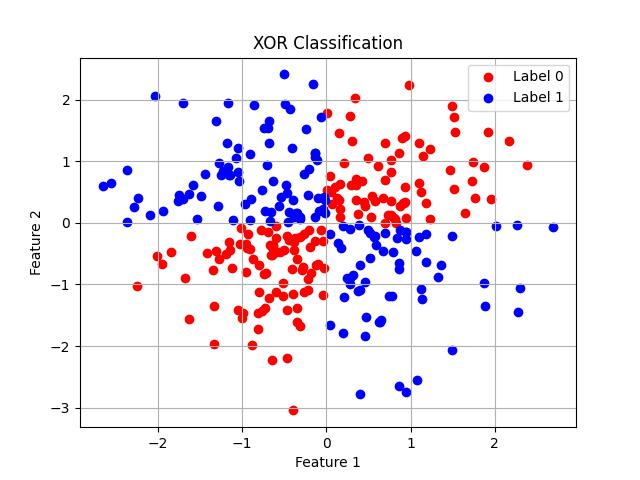
\includegraphics[width=0.5\textwidth]{lab3/XOR_data.jpg}
    \caption{异或(XOR)问题}
    \label{xor}
\end{figure}

本题中我们将通过实验了解核函数的选择对于SVM解决非线性问题的影响. 请使用\href{https://scikit-learn.org/stable/modules/generated/sklearn.svm.SVC.html}{ sklearn包中的SVM分类器}完成下述实验: 
\begin{enumerate}
    \item[(1)] \textbf{[6pts]} 请分别训练线性核SVM分类器和高斯核(RBF核) SVM分类器, 并绘制出各自的决策边界.
    \item[(2)] \textbf{[6pts]} sklearn还允许自定义核函数, 参考\texttt{lab3/svm\_kernel\_custom.py}的用法, 编写核函数$\kappa(\vx, \vx') = \frac{1}{1+\|\vx-\vx'\|_2^{2}}$, 训练该核函数的SVM分类器, 并绘制出决策边界. 
\end{enumerate} 
具体的实验要求可以参考\texttt{lab3/svm\_kernel.py}的\texttt{main}部分. 请将\texttt{lab3/svm\_kernel\_solution.py}中的代码和三个核函数分别对应的决策边界图提交至下方的解答处. 
\vspace{5pt}

最后, 请直接回答 \textbf{[3pts]}:三个核函数, 各自能够解决异或(XOR)分类问题吗?

\begin{solution}
    此处用于写解答(中英文均可)
    
    求解代码为:
    \lstinputlisting[language=Python]{lab3/svm_kernel_solution.py}
    
    决策边界为:
     \begin{figure}[h]
        \centering
         \begin{subfigure}[b]{0.3\textwidth}
             \includegraphics[width=\textwidth]{clf_linear.jpg}
             \caption{clf\_linear}
         \end{subfigure}
         \begin{subfigure}[b]{0.3\textwidth}
             \includegraphics[width=\textwidth]{clf_rbf.jpg}
             \caption{clf\_rbf}
         \end{subfigure}
        \begin{subfigure}[b]{0.3\textwidth}
            \includegraphics[width=\textwidth]{clf_custom.jpg}
           \caption{clf\_custom}
        \end{subfigure}
     \end{figure}
        
    能否解决异或(XOR)分类问题:线性核函数不能解决,高斯核函数和自定义核函数可以解决.
\end{solution}

\newpage

\section{[30pts] Maximum Likelihood Estimation}
给定由$m$个样本组成的训练集$D=\left\{(\vx_1,y_1),(\vx_2,y_2),\cdots,(\vx_m,y_m)\right\}$, 其中$\vx_i\in\mathbb{R}^{d}$是第$i$个示例, $y_i\in\mathbb{R}$是对应的实值标记. 令$\mX\in\mathbb{R}^{m\times d}$表示整个训练集中所有样本特征构成的矩阵, 并令$\vy\in\mathbb{R}^{m}$表示训练集中所有样本标记构成的向量. 线性回归的目标是寻找一个参数向量$\vw\in\mathbb{R}^{d}$, 使得在训练集上模型预测的结果和真实标记之间的差距最小. 对于一个样本$\vx$, 线性回归给出的预测为$\hat{y}=\vw^\top\vx$,\footnote{本题不考虑偏移$b$, 可参考教材第3章将偏移$b$吸收进$\vw$. } 它与真实标记$y$之间的差距可以用平方损失$(\hat{y}-y)^2$来描述. 因此, 在整个训练集上最小化损失函数的过程可以写作如下的优化问题:
\begin{equation}
    \vw^\star=\underset{\vw}{\arg\min}\|\mX\vw-\vy\|_2^2
    \label{linear_regression_target}
\end{equation}
\begin{enumerate}
    \item[(1)] \textbf{[8pts]} 考虑这样一种概率观点: 样本$\vx$的标记$y$是从一个高斯分布$\mathcal{N}(\vw^\top\vx,\sigma^2)$中采样得到的. 这个高斯分布的均值由样本特征$\vx$和模型参数$\vw$共同决定, 而方差是一个额外的参数$\sigma^2$. 基于这种概率观点, 我们可以基于观测数据对高斯分布中的参数$\vw$做极大似然估计. 请证明: $\vw$的极大似然估计结果$\vw_{\mathrm{MLE}}$与式~\eqref{linear_regression_target}~中的$\vw^\star$相等;
	
    \item[(2)] \textbf{[9pts]} 极大似然估计容易过拟合, 一种常见的解决办法是采用最大后验估计: 沿着上一小问的思路, 现在我们希望在概率建模下对参数$\vw$做最大后验估计. 为此, 引入参数$\vw$上的先验$p(\vw)=\mathcal{N}(\vzero,\lambda\mat{I})$. 其中, 均值$\vzero$是$d$维的全$0$向量, $\mI$是$d$维单位矩阵, $\lambda>0$是一个控制方差的超参数. 现在, 请推导对$\vw$做最大后验估计的目标函数, 并讨论一下该结果与``带有$\mathrm{L}_2$范数正则项的线性回归"之间的关系;
	
    \item[(3)] \textbf{[9pts]} 沿着上一小问的思路, 我们尝试给参数$\vw$施加一个拉普拉斯先验. 简便起见, 我们假设参数$\vw$的$d$个维度之间是独立的, 且每一维都服从$0$均值的一元拉普拉斯分布, 即:
    \begin{equation}
	\begin{aligned}
	& p(\vw)=\prod_{j=1}^{d}p(w_j)\;, \\
	& p(w_j)=\mathrm{Lap}(w_j\mid 0,\lambda),\;j=1,2,\ldots,d\;.
	\end{aligned}
    \end{equation}
    请推导对$\vw$做最大后验估计的目标函数, 并讨论一下该结果与``带有$\mathrm{L}_1$范数正则项的线性回归"之间的关系;

    \textit{Note: 由参数$\mu$, $\lambda$确定的一元拉普拉斯分布的概率密度函数为:}
    \begin{equation}
	\mathrm{Lap}(w\mid\mu,\lambda)=\frac{1}{2\lambda}\exp\left(-\frac{|w-\mu|}{\lambda}\right)\;.
    \end{equation}	
    \item[(4)] \textbf{[4pts]} 基于(2)和(3)的结果, 从概率角度讨论为什么$\mathrm{L}_{1}$范数能使模型参数更稀疏.
\end{enumerate}

\begin{solution}
此处用于写解答(中英文均可)
~\\
(1) 对于高斯分布,其对数似然函数为:
$$\begin{aligned}
\log p(\vy|\vw) &= \log \prod_{i=1}^{m} \mathcal{N}(y_i|\vw^\top\vx_i,\sigma^2) \\n&= \sum_{i=1}^{m} \log \mathcal{N}(y_i|\vw^\top\vx_i,\sigma^2) \\n&= \frac{m}{2}\log(2\pi\sigma^2) + \frac{1}{2\sigma^2}\|\mX\vw-\vy\|_2^2
\end{aligned}$$
要找到一个w使得$\ln L(\w|\X,\y)$最大, 即$\w_{MLE} = \underset{\bm w}{\arg\max} \ln L(\w|\X,\y)$
前一项显然与w无关,后一项和式(4.1)成反比.
最大化对数似然函数等价于最小化平方损失函数。因此,$\vw_{\mathrm{MLE}}$与式~\eqref{linear_regression_target}~中的$\vw^\star$显然相等。

(2) 由题意知,此分布的概率密度函数为:
\[ p(\vw) = \frac{1}{(2\pi\lambda)^{d/2}} \exp \left( -\frac{\|\vw\|^2}{2\lambda} \right) \]

我们需要计算参数$\vw$的后验分布$p(\vw|\y,\X)$,根据贝叶斯公式:
\[ p(\vw|\y,\X) = \frac{p(\y|\X,\vw)p(\vw)}{p(\y|\X)} \]
\[ \log p(\vw|\y,\X) = \log p(\y|\X,\vw) + \log p(\vw) - \log p(\y|\X) = \log p(\y|\X,\vw) + \log p(\vw) \]
\[ \log p(\vw|\y,\X) = -\frac{m}{2} \log(2\pi\sigma^2) - \frac{1}{2\sigma^2} \sum_{i=1}^{m} (y_i - \vw^T x_i)^2 - \frac{d}{2} \log(2\pi\lambda) - \frac{1}{2\lambda} \|\vw\|^2 \]

\[ \vw_{\mathrm{MAP}} = \underset{\vw}{\arg\min} \left( \frac{1}{2\sigma^2} \sum_{i=1}^{m} (y_i - \vw^T \mathbf{x}_i)^2 + \frac{1}{2\lambda} \|\vw\|^2 \right) \]
\[ \vw_{\mathrm{MAP}} = \underset{\vw}{\arg\min} \left( \|\X\vw - \y\|^2 + \sigma^2 \lambda \|\vw\|^2 \right) \]

这个目标函数正是带有$\mathrm{L}_{2}$正则项的线性回归,其正则化系数为$\frac{\sigma^2}{\lambda}$.

(3) 推导过程:\\
$p(\vw)=\prod_{j=1}^{d} p(\vw_j), \quad p(\vw_j)=\text{Lap}(\vw_j|0,\lambda)=\frac{1}{2\lambda} \exp\left(-\frac{|\vw_j|}{\lambda}\right)$\\
$\log p(\vw|\y,\X) = \log p(\y|\X,\vw) + \log p(\vw) - \log p(\y|\X) = \log p(\y|\X,\vw) + \log p(\vw)$

$\log p(\vw|\y,\X) = -\frac{m}{2} \log(2\pi\sigma^2) - \frac{1}{2\sigma^2} \sum_{i=1}^{m} (y_i - \vw^{\top}\x_i)^2 + \sum_{j=1}^{d} \log \frac{1}{2\lambda} \exp(-|w_j|/\lambda)$\\
$\log p(\vw|\y,\X) = -\frac{m}{2} \log(2\pi\sigma^2) - \frac{1}{2\sigma^2} \sum_{i=1}^{m} (y_i - \vw^{\top}\x_i)^2 - \sum_{j=1}^{d} \log(2\lambda) + |\vw_j|/\lambda$\\
$\vw_{\text{MAP}} = \underset{\vw}{\arg\min} \|\X\vw - \y\|_2^2 + \frac{2\sigma^2}{\lambda} \|\vw\|_1$\\
这个目标函数正是带有$\mathrm{L}_{1}$正则项的线性回归,其正则化系数为$\frac{2 \sigma^2}{\lambda}$.\\
(4) 从概率角度来说,$\mathrm{L}_{1}$范数对应于拉普拉斯分布,这种分布鼓励模型参数中的许多值接近零,因为拉普拉斯分布在0处的陡峭,可以使模型参数更稀疏。它对参数的绝对值进行惩罚,使得参数更倾向于取较小的值。这样,在最大后验估计中,参数的先验分布会偏向于较小的值,从而使得模型参数更加稀疏。
\end{solution}

\newpage
\section*{Acknowledgments}
允许与其他同样未完成作业的同学讨论作业的内容, 但需在此注明并加以致谢; 如在作业过程中, 参考了互联网上的资料 (包括生成式模型的结果), 且对完成作业有帮助的, 亦需注明并致谢.

\end{document}
